\documentclass[letter,12pt]{article}
\usepackage[utf8]{inputenc}
\usepackage{fullpage}
\usepackage{graphicx}
\usepackage{datetime}

\newdateformat{mydate}{\THEDAY\space \shortmonthname[\THEMONTH] \THEYEAR}

\title{Switched LANs Lab Report}
\author{Sam Harkness}
\date{\mydate\today}

\begin{document}

%\maketitle

\begin{flushleft}
	\begin{tabular}{l l}
		To: & Prof. Richard Wolff \\
		From: & Sam Harkness \\
		Regarding: & Switched LANs Lab Report \\
		Date: & \mydate\today
	\end{tabular}
\end{flushleft}



\begin{abstract}
	\noindent The objective of this lab is to demonstrate the implementation of switched local area networks. For this exercise, 4 scenarios were created:
	\begin{enumerate}
		\item HubOnly: 16 Ethernet workstations are networked together using a 16-port Ethernet hub. The entire network uses the 10BaseT Ethernet standard.
		\item HubAndSwitch: The network of HubOnly has been divided into 2 hubs of 8 workstations connected with an Ethernet switch.  The entire network uses the 10BaseT Ethernet standard.
		\item SwitchOnly: The Ethernet hub of HubOnly is replaced with an Ethernet switch.
		\item TwoSwitches: The network is divided into 2 switches of 8 workstations connected together by 10BaseT.
	\end{enumerate}
\end{abstract}

\section{Question 1:}
	As you can see in Figure~\ref{Ethernet_Delay}, the delay in the HubAndSwitch network is much less than in the OnlyHub network.  This is due to the unsophisticated nature of Ethernet hubs. A hub does not examine or manage any of the traffic that comes through it: any packet entering any port is rebroadcast on all other ports. Consequently, packet collisions are more frequent, as can be seen in Figure~\ref{Ethernet_Collisions}.  By separating the network into 2 switched hubs, the collision domain is cut in half, significanlty reducing the number of packets that need to be retransmitted, which in turn significantly reduces the average delay of the network.

	\begin{figure}[h!]
		\centering
			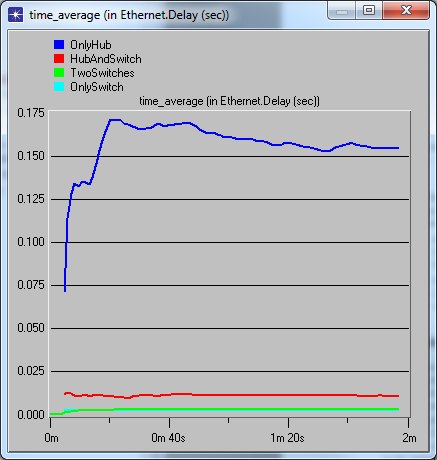
\includegraphics[scale=0.6]{Ethernet_Delay.png}
		\caption{Ethernet Delay}
		\label{Ethernet_Delay}
	\end{figure}
	
	\begin{figure}[h!]
		\centering
		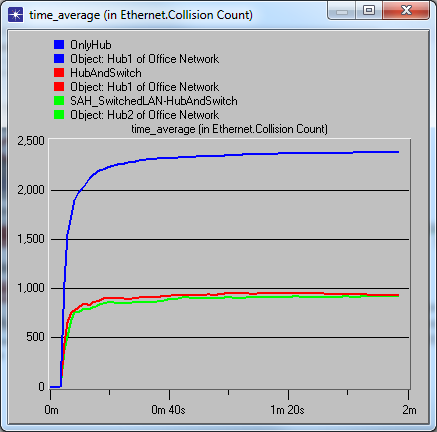
\includegraphics[scale=0.6]{Ethernet_Collision.png}
		\caption{Ethernet Collision}
		\label{Ethernet_Collisions}
	\end{figure}
	
\pagebreak

\section{Question 2:}
	The collision count of the Ethernet switch cannot be analyzed, because switches have no collisions! Switches manage all of the traffic that pass through it.  Packets are only rebroadcast towards the destination on the packet, nowhere else.  Instead of collisions occurring when multiple packets arrive at the same time, excess packets are put onto a buffer.  However, if the buffer overflows then packets are 'dropped', which requires re-transmittal of packets.

\section{Question 3:}
	Figure~\ref{Throughput} shows the throughput of the network in the 10BaseT connection to workstation 0. It is plain to see the HubOnly network is heavily affected by collisions.  Any of the other network configurations greatly increases throughput and decreases delay, as can be seen in Figure~\ref{Ethernet_Delay}. \\
	
	\noindent Figures \ref{Traffic_Received} and \ref{Traffic_Sent}, show the traffic generated is higher, and traffic received lower, in the HubOnly network. This is due to packet collisions and the necessary packet re-transmittals.
	
	\begin{figure}[h!]
		\centering
		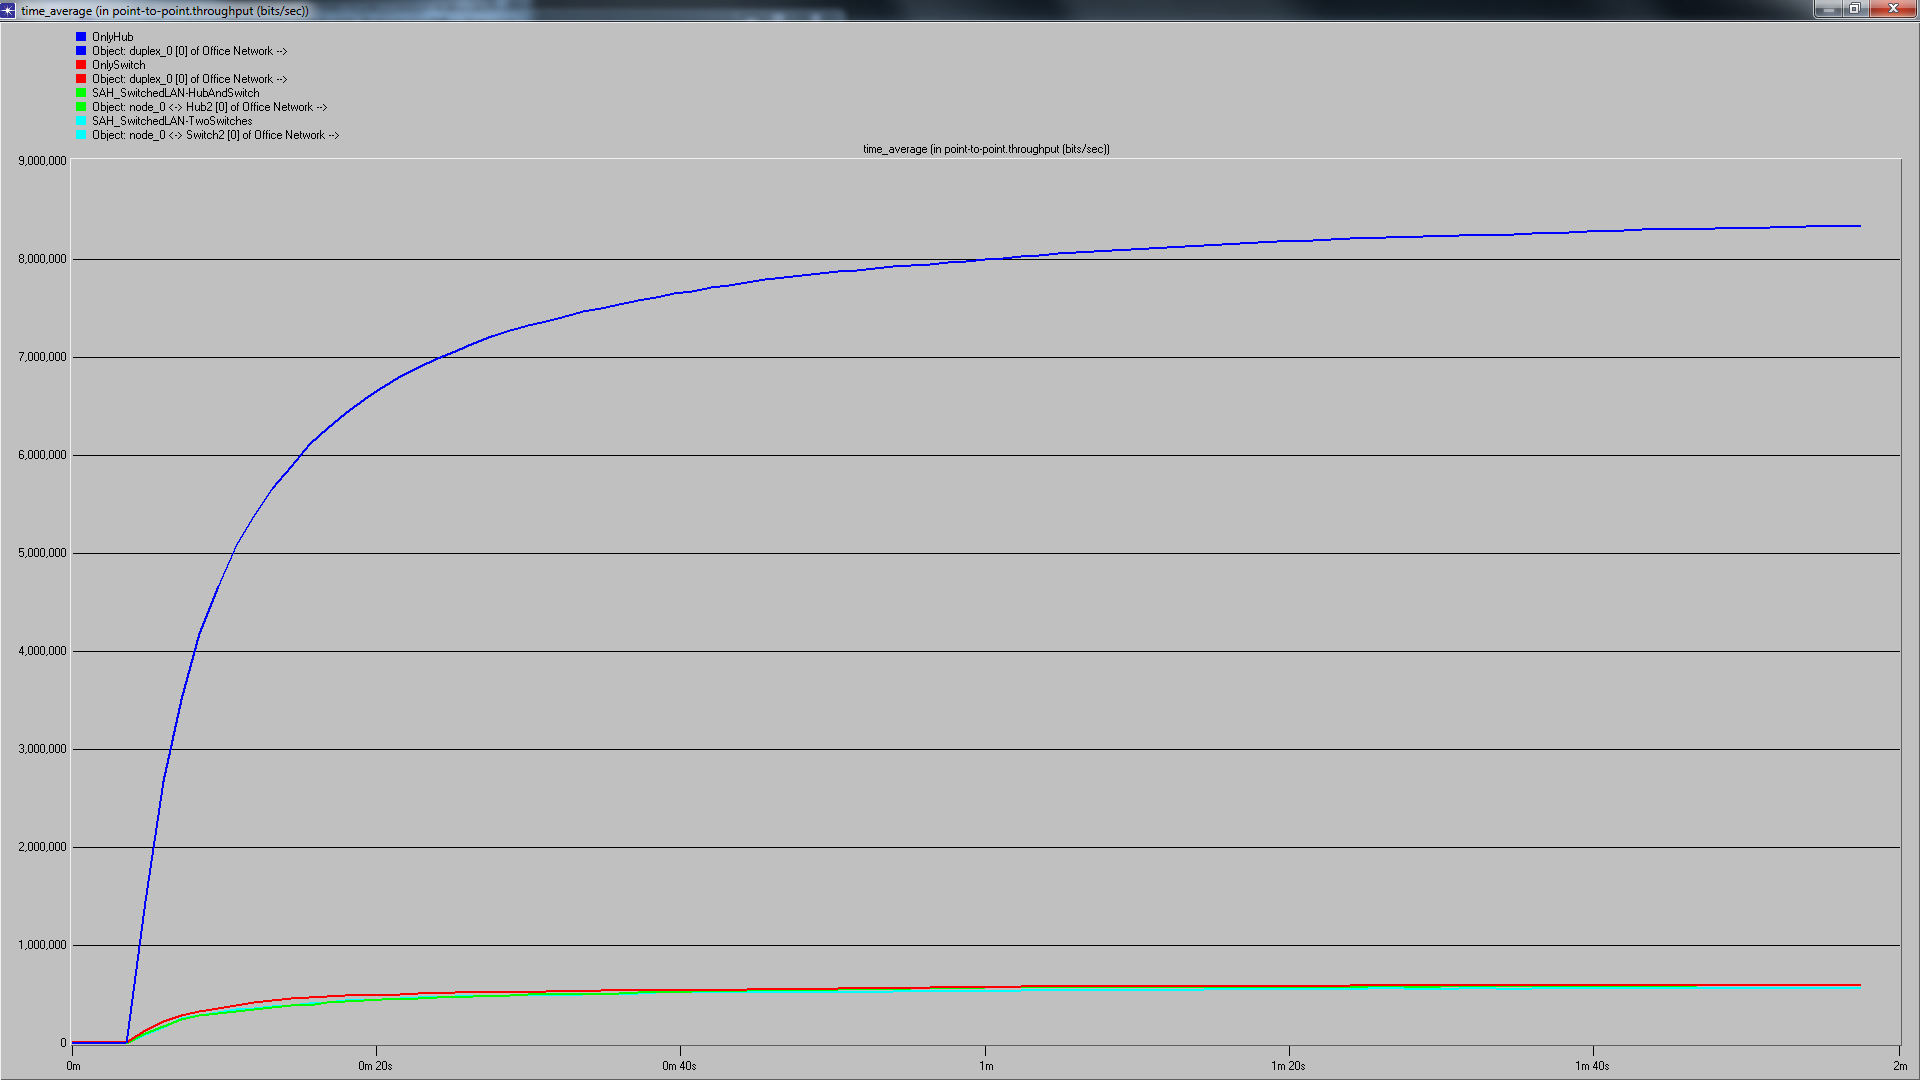
\includegraphics[width=\linewidth]{Throughput.png}
		\caption{Throughput}
		\label{Throughput}
	\end{figure}
	

\begin{figure}[h]
	\centering
	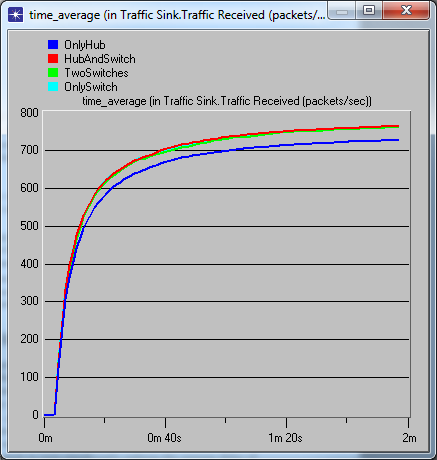
\includegraphics[scale=0.6]{Traffic_Received.png}
	\caption{Traffic Received}
	\label{Traffic_Received}
\end{figure}

\begin{figure}[h]
	\centering
	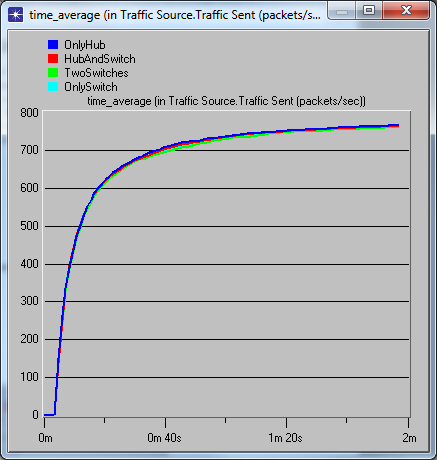
\includegraphics[scale=0.6]{Traffic_Sent.png}
	\caption{Traffic Sent}
	\label{Traffic_Sent}
\end{figure}

\end{document}
